\documentclass[11pt]{article}

% ---------------------------------------------------------------
% Critical assessment of the GDTW sequence-similarity method:
% four structural weaknesses, evidence, and proposed remedies.
% Condensed edition -- same content, no restatement.
% ---------------------------------------------------------------

\usepackage[margin=1in]{geometry}
\usepackage{amsmath,amssymb}
\usepackage{enumitem}
\usepackage{booktabs}
\usepackage{float}
\usepackage{graphicx}
\usepackage{xcolor}
\usepackage[colorlinks=true,linkcolor=blue,citecolor=teal,urlcolor=blue]{hyperref}
\usepackage{tabularx}
\usepackage{caption}

\captionsetup{font=small}
\setlength{\emergencystretch}{3em}
\setlist{itemsep=1pt,parsep=1pt,topsep=3pt}
\newcommand{\code}[1]{\texttt{\small #1}}
\newcommand{\finding}[1]{\textcolor{red}{\textbf{#1}}}
\setcounter{tocdepth}{1}

\title{\textbf{Four Structural Weaknesses of the GDTW Similarity Metric}\\
\large Diagnosis, Empirical Evidence, and Proposed Remedies}
\author{Yuli Tshuva}
\date{August 2026}

\begin{document}
\maketitle
\vspace{-1.5em}

\begin{abstract}
\noindent
Four known weaknesses of the segment-based similarity metric (\emph{GDTW}): (i) the
change-point detector is a heuristic stack with no stability guarantee; (ii) the merge rule
is governed by an unmotivated constant; (iii) the segment representation misrepresents scale
on both axes; (iv) the paradigm collects human judgements but the model contains no learning.
Each is diagnosed against the implementation, measured on the project corpus (10{,}000 mined
stock-price sequences), and matched to a remedy from the literature. Three further defects
found during the audit are in \S\ref{sec:cross}; \S\ref{sec:roadmap} ranks all
recommendations. \textbf{Reading order for the author:} \S\ref{sec:roadmap} (the whole report
as a ranked list), then \S\ref{sec:cross}, then \S\ref{sec:learning}.
\end{abstract}

\vspace{-0.5em}
{\small\tableofcontents}

% ===============================================================
\section{The method under review}
% ===============================================================
GDTW (\code{seq\_sim\_alg.py:seq\_distance}) min--max normalises each sequence
(\code{normalize\_sequence}); segments it at change points
(\code{change\_points\_detection}); maps each segment to a 12-dimensional feature vector
$\phi(s)$ (\code{extract\_segment\_features}), standardised by hard-coded constants and
scaled componentwise by weights $w \in \Delta^{11}$; then aligns the two segment chains with
a merge-aware dynamic program (\code{dtw\_merge}). A merge step consuming $d_i$ segments of
$f$ and $d_j$ of $g$ costs
\begin{equation}
\label{eq:cost}
\begin{split}
  \mathrm{cost} \;&=\; \frac{L_x + L_y}{2}\,\big( \Delta_{ij} + P_{ij} \big), \qquad
  \Delta_{ij} \;=\; \underbrace{\big\lVert \mu(X_{i-d_i:i}) - \mu(Y_{j-d_j:j}) \big\rVert_2}_{\text{merged feature distance}}, \\[2pt]
  P_{ij} \;&=\; \underbrace{(\lambda_1 - 3\lambda_2 \rho_x)(d_i-1) \;+\; (\lambda_1 - 3\lambda_2 \rho_y)(d_j-1)}_{\text{merge penalty}},
\end{split}
\end{equation}
with $L_x,L_y$ the relative durations, $\mu$ the feature-merge operator
(\code{merge\_sequence}), $\rho$ a correlation over trend features
(\code{features\_correlation}), and $\lambda_1,\lambda_2$ the mean and s.d.\ of the
segment-to-segment distance matrix. All measurements below use
\code{data/six\_cps\_sequences.npz} (10{,}000 sequences, length 1000, mean 5.93 change
points); scripts are in \code{reports/diagnostics/}.

% ===============================================================
\section{Weakness 1: the change-point detector}
\label{sec:cpd}
% ===============================================================
\code{change\_points\_detection} chains five heuristics, each with its own constant:
a ternary sign map of $f'$ at $\tau = 0.10\cdot\mathrm{der\_amp}$ where
$\mathrm{der\_amp} = \tfrac12(\max f' - \min f')$, summed with a second map at $\tau/3$
(\code{utils.py:204--205}); \code{feature\_points} (emits a point pair when the running sign
window exceeds 2\% of length); \code{find\_local\_extrema} (smoothed-derivative zero
crossings, 5\% prominence filter); \code{drop\_false\_extrema}; and
\code{merge\_nearby\_points} (removes points closer than $\max(5,1\%)$, then midpoint-merges
points within 1\% in height).

\paragraph{(a) No objective.} Nothing is optimised. There is no cost function whose minimiser
is the returned segmentation, hence no notion of correctness, no way to compare two
segmentations, and no fit-versus-complexity trade-off. Each stage greedily edits the previous
one's output; early errors are unrecoverable.

\paragraph{(b) The governing threshold is maximally non-robust.} $\tau \propto \max f' - \min
f'$ --- the derivative \emph{range}, fixed by 2 samples out of 999, with unbounded
sensitivity to one outlier. It governs what counts as ``changing'' everywhere, so one noisy
sample rescales the whole segmentation. The same statistic recurs in
\code{extract\_segment\_features} (\code{utils.py:316}), so the \emph{descriptors} inherit
the fragility.

\paragraph{(c) Six unidentified constants.} 2\% (segment percentage), 10\% (change
threshold), the $\tau/3$ split, 5\% (prominence), 1\% (minimum distance), 1\% (height merge).
None fitted, none with a sensitivity analysis.

\paragraph{(d) One third of the detector is dead code.} \code{find\_local\_extrema}
(\code{utils.py:213}) feeds a list \code{combined} (\code{utils.py:217--232}) that is never
read --- line 234 proceeds from \code{signs\_fps}. Verified: stubbing
\code{find\_local\_extrema} to return \code{[]} leaves segmentation \finding{bit-identical on
300/300 sequences}. About 40 lines, including all prominence logic, affect no published
result.

\subsection{Evidence}
60 random sequences, perturbed and re-segmented. Hausdorff = boundary displacement as \% of
sequence length.

\begin{table}[H]
\centering\small
\caption{Segmentation stability under perturbation (mean 5.93 change points).}
\begin{tabular}{lrrrr}
\toprule
Perturbation & \% seq.\ with & mean & median & p90 \\
             & changed $K$   & $|\Delta K|$ & Hausdorff & Hausdorff \\
\midrule
Gaussian noise $\sigma=0.005$ & \finding{100.0\%} & \finding{3.92} & \finding{41.8\%} & 48.6\% \\
Gaussian noise $\sigma=0.01$  & 100.0\% & 3.92 & 41.8\% & 48.6\% \\
Time resample $\times 1.05$   & 0.0\%   & 0.00 & 0.1\%  & 0.3\% \\
Time shift, 1\% of length     & 11.7\%  & 0.12 & 1.0\%  & 2.2\% \\
Amplitude rescale $\times0.98$& 0.0\%   & 0.00 & 0.0\%  & 0.0\% \\
\midrule
\emph{PELT (\code{ruptures}, $\ell_2$), noise $\sigma=0.01$} & 32.0\% & 0.40 & 1.5\% & --- \\
\bottomrule
\end{tabular}
\end{table}

\vspace{-0.5em}
A 0.5\%-of-range perturbation --- invisible at plotting resolution --- changes the segment
count in \emph{every} sequence, by two thirds of the mean count, and displaces boundaries by
42\% of the sequence length. That is a different segmentation, not a perturbed one. PELT
under twice the noise is $10\times$ more stable in count, $28\times$ in localisation.

\paragraph{Mechanism.} Diagnosis (b) confirmed: under $\sigma=0.005$, $\mathrm{der\_amp}$
inflates by a median factor of \textbf{6.7} (p90: 10.9), $\tau$ with it, and the fraction of
samples deemed ``not changing'' rises from 13.3\% to 26.0\% --- the detector goes half blind.
A robust scale (derivative IQR) inflates only $4.15\times$.

\begin{figure}[H]
\centering
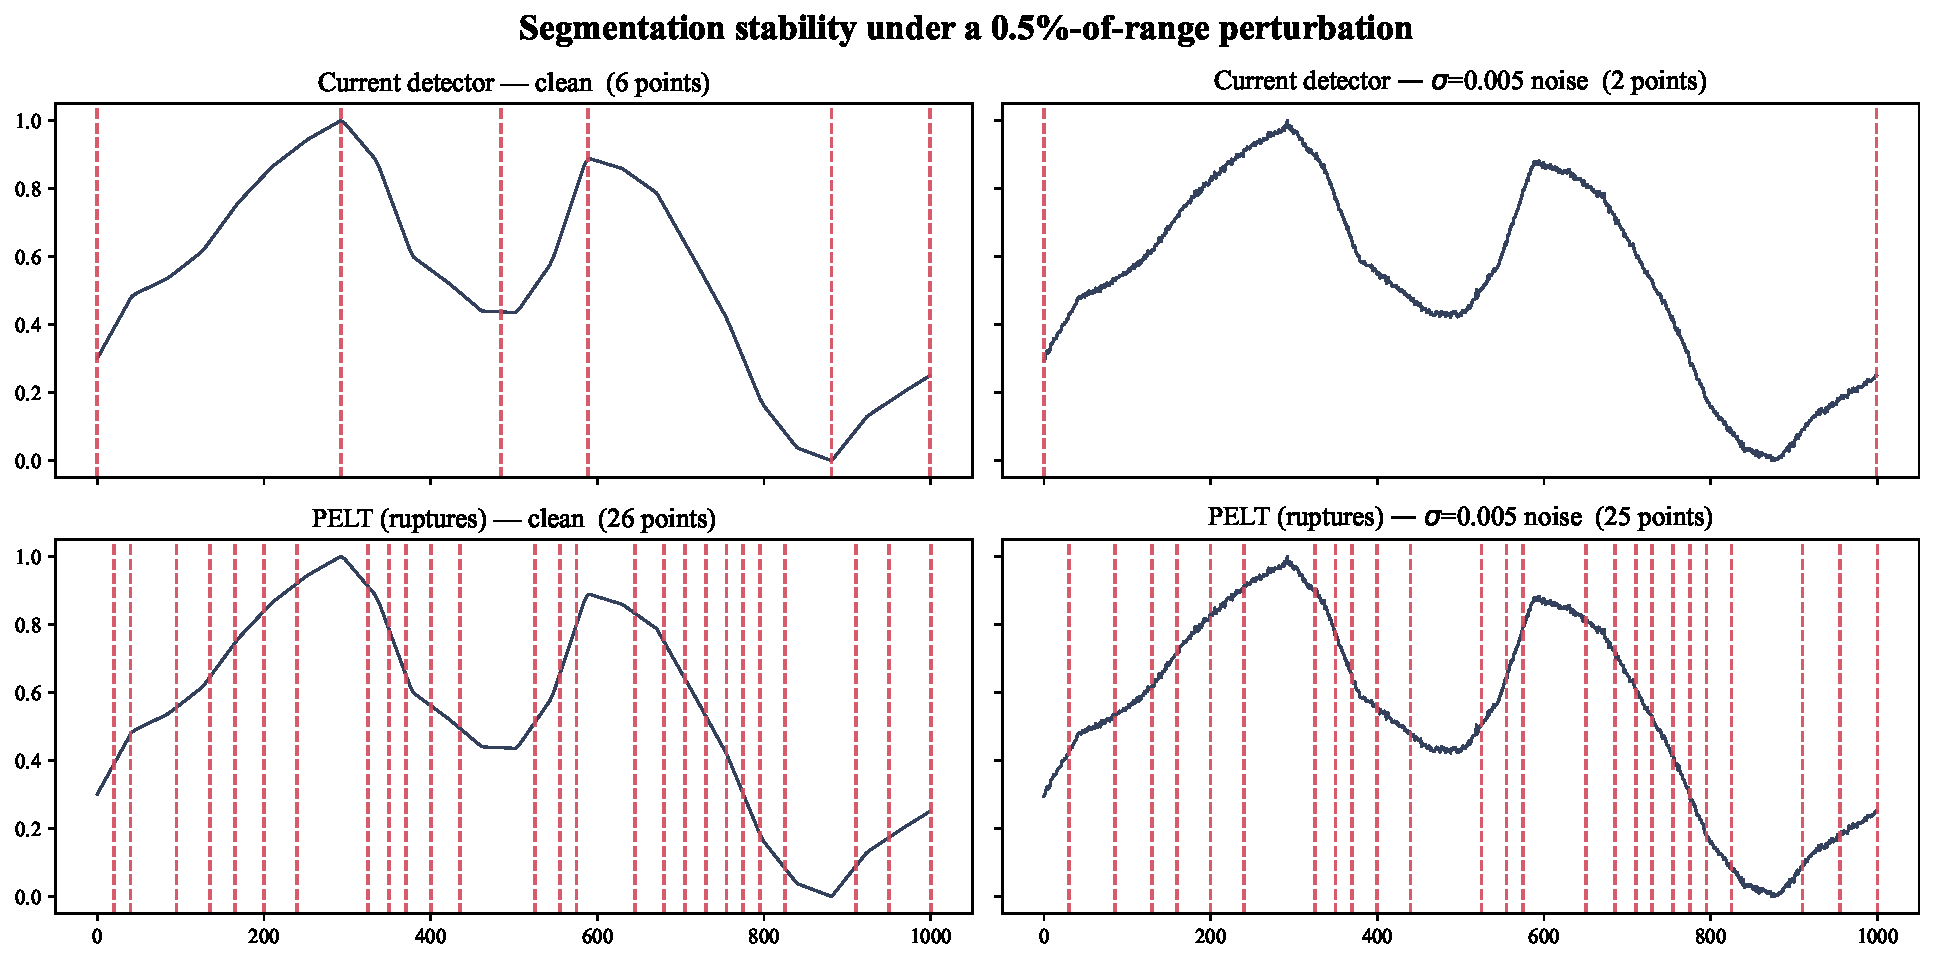
\includegraphics[width=0.92\textwidth]{figs/fig_cp_stability.pdf}
\caption{Top: current detector, clean and perturbed --- six change points collapse to two.
Bottom: PELT on the same signals, $26 \to 25$. PELT's penalty ($\beta=0.05$) was not tuned
for parsimony, so this compares \emph{stability}, not granularity.}
\label{fig:cpstab}
\end{figure}

\subsection{Remedy}
The field formulates segmentation as \emph{penalised model selection}: a cost function, a
search strategy, a constraint on the number of changes [3]. The \code{ruptures} package is
already in \code{requirements.txt} but unused.

\begin{enumerate}[leftmargin=*]
  \item \textbf{Replace the stack with $\ell_1$ trend filtering [6]} ---
  $\min_x \tfrac12\lVert y-x\rVert_2^2 + \lambda\lVert D^{(2)}x\rVert_1$, convex, solution
  exactly piecewise linear with knots at the kinks. Best fit to GDTW's needs: it denoises
  \emph{and} segments in one step, returns the per-segment trend model that
  \S\ref{sec:merge} needs, has one parameter with a known regularisation path, and being
  convex is unique and stable. Alternative: \textbf{PELT [4]} with a piecewise-linear cost
  (\code{CostLinear}, or $\ell_2$ on the derivative), exact in expected linear time, one
  parameter $\beta$ settable by BIC/MDL or learned (\S\ref{sec:learning}). For outlier
  robustness see Fearnhead \& Rigaill [5], the principled version of what (b) gets wrong.
  FLUSS/FLOSS [8] is domain-agnostic but detects \emph{regime} change via motif recurrence
  --- a different notion from visual gestures; not recommended here.
  \item \textbf{Keep PIP [1] as comparator} --- recursive maximal-deviation-from-chord
  selection, deterministic, one parameter, yields a \emph{nested hierarchy}, and was designed
  for human-perceived shape in financial charts. If conclusions survive swapping the
  segmenter, the contribution is the alignment, which strengthens the paper. Its hierarchy
  also turns \S\ref{sec:merge}'s merge decision into a choice of \emph{level}.
  \item \textbf{Delete or wire in the dead branch}, then re-run every published result.
  \item \textbf{Report stability as a metric}: median Hausdorff and $|\Delta K|$ at
  $\sigma \in \{0.005,0.01,0.02\}$. A metric claiming to model human perception cannot have a
  representation that moves under noise humans cannot see.
\end{enumerate}

% ===============================================================
\section{Weakness 2: misrepresentation of scale}
\label{sec:scale}
% ===============================================================

\paragraph{(a) Features are dimensionally inhomogeneous in time.} With $\Delta t$ the
sampling interval: \code{mean\_curvature} $= \overline{|\Delta^2 s|}$ scales as
$\mathcal{O}(\Delta t^{2})$; \code{mean\_diff} and \code{mean\_abs\_diff} as
$\mathcal{O}(\Delta t)$; \code{sum\_abs\_diff}, \code{amplitude}, \code{mean\_value},
\code{length} as $\mathcal{O}(1)$. So resampling a segment without touching its drawn shape
changes its descriptor. Resampling a real segment (192 samples, sequence 3050) by
$\{0.5,1,2,4\}$, rescaling its container identically so the rendering is unchanged:

\begin{table}[H]
\centering\small
\caption{One segment at four sampling resolutions; the shape is identical throughout.}
\begin{tabular}{lrrrrr}
\toprule
Feature & $\times0.5$ & $\times1$ & $\times2$ & $\times4$ & max/min \\
\midrule
\code{mean\_curvature} & 0.000260 & 0.000064 & 0.000016 & 0.000004 & \finding{65.7} \\
\code{mean\_diff}      & $-$0.00592 & $-$0.00294 & $-$0.00147 & $-$0.00073 & \finding{8.07} \\
\code{mean\_abs\_diff} & 0.00592 & 0.00294 & 0.00147 & 0.00073 & \finding{8.07} \\
\code{amplitude} \emph{(and the 8 others)} & 0.56232 & 0.56232 & 0.56232 & 0.56232 & 1.00 \\
\bottomrule
\end{tabular}
\end{table}

\vspace{-0.5em}
Observed ratios match the predicted exponents exactly ($8^1 = 8.07$, $8^2 = 64 \approx
65.7$). This is masked only because \code{mine\_data.py} interpolates everything to 1000
points: \finding{the pipeline is self-consistent solely because of a preprocessing step a
real deployment would not have}. Any variable-length or multi-resolution use breaks it
silently, and sampling-rate invariance --- required of a perceptual metric --- cannot be
claimed.

\paragraph{(b) Global normalisation makes segment scale context-dependent.} Because
\code{normalize\_sequence} min--max scales the \emph{whole} sequence, a segment's
\code{amplitude} and \code{mean\_value} measure it against extremes set by parts of the
sequence it has nothing to do with. The same 200-sample motif placed before four different
tails:

\begin{table}[H]
\centering\small
\caption{One motif, four contexts.}
\begin{tabular}{lrrrr}
\toprule
Tail slope & 0.1 & 0.5 & 2.0 & 5.0 \\
\midrule
\code{amplitude} of the motif   & 1.0000 & 0.4615 & 0.1395 & \finding{0.0583} \\
\code{mean\_value} of the motif & 0.5000 & 0.2308 & 0.0698 & 0.0291 \\
\bottomrule
\end{tabular}
\end{table}

\vspace{-0.5em}
A $17\times$ swing with the motif untouched (Fig.~\ref{fig:scalectx}). Min--max is also
non-robust: one outlier compresses everything else. The trend fractions are unaffected
\emph{here} only because the tail is monotone; in general they move too, since their
threshold derives from the global $\mathrm{der\_amp}$.

\begin{figure}[H]
\centering
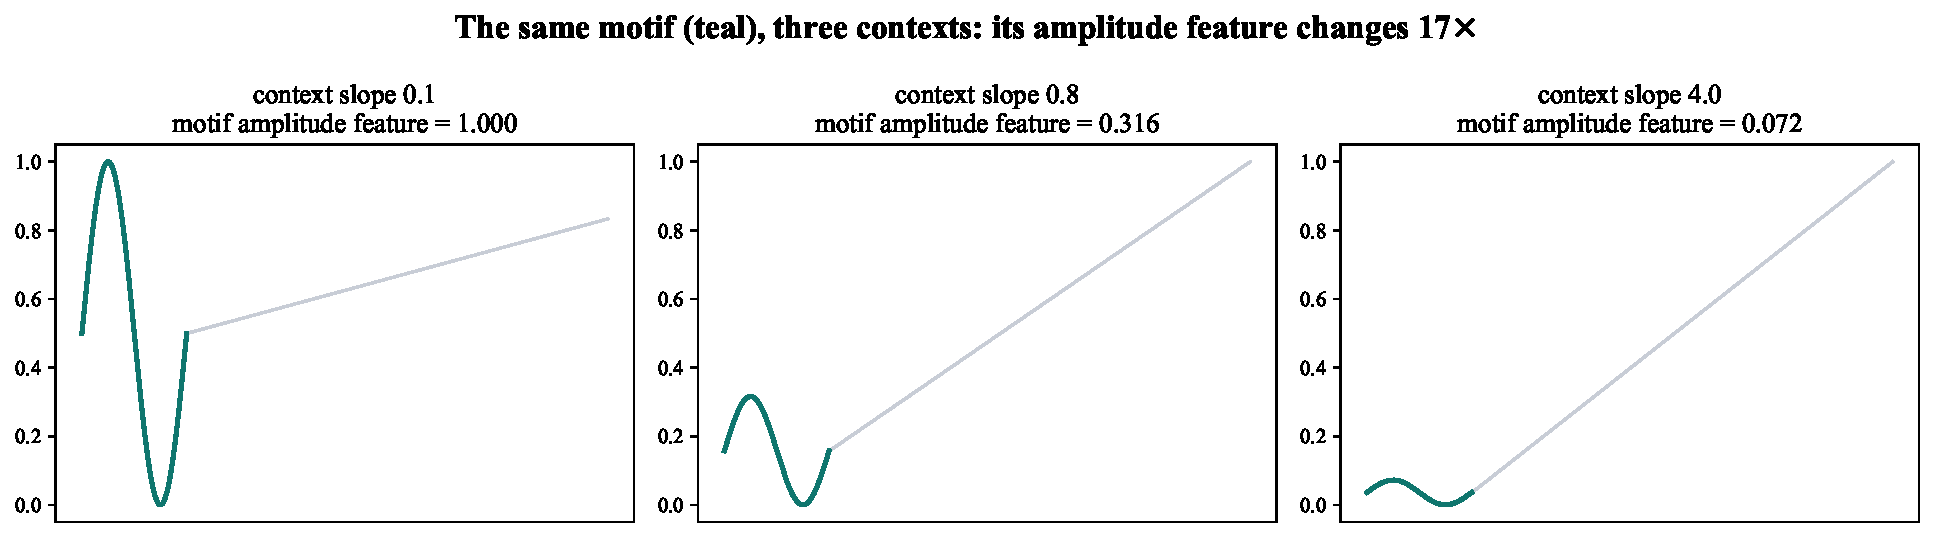
\includegraphics[width=0.92\textwidth]{figs/fig_scale_context.pdf}
\caption{The identical motif (teal) in three contexts. Its \code{amplitude} feature --- which
the metric treats as a property of the motif --- is a property of the tail.}
\label{fig:scalectx}
\end{figure}

\paragraph{(c) Duration is double-counted, and the features are collinear.} In
Eq.~\ref{eq:cost} relative duration enters \emph{multiplicatively} as $(L_x+L_y)/2$
\emph{and} additively as \code{length} inside the norm, with no stated semantics for the
composite. Over 1489 real segments:

\begin{table}[H]
\centering\small
\begin{tabular}{lrlr}
\toprule
Pair & $r$ & Pair & $r$ \\
\midrule
\code{sum\_abs\_diff} $\sim$ \code{amplitude} & \finding{$+0.997$} & \code{mean\_diff} $\sim$ \code{sharp\_increasing} & $+0.844$ \\
\code{sum\_abs\_diff} $\sim$ \code{length}    & $+0.847$ & \code{mean\_diff} $\sim$ \code{sharp\_decreasing} & $-0.838$ \\
\code{amplitude} $\sim$ \code{length}         & $+0.845$ & $|\code{mean\_diff}\times\code{length}| \sim \code{amplitude}$ & \finding{$+1.000$} \\
\bottomrule
\end{tabular}
\end{table}

\vspace{-0.5em}
Segments are near-monotone by construction, so total variation \emph{is} amplitude
($r=0.997$) and slope $\times$ duration \emph{is} amplitude exactly ($r=1.000$). The twelve
``independent perceptual axes'' carry 95\% of their variance in \finding{7 components}, with
condition number $4\times10^{12}$. Consequence for \S\ref{sec:learning}: a diagonal weight
vector over collinear features is \textbf{not identifiable}.

\paragraph{(d) No aspect ratio.} Humans judge a \emph{rendering}, and perceived slope depends
on aspect ratio --- ``banking to $45^\circ$'' [18], refined empirically by [19]; Gogolou et
al.\ [20] show similarity perception in time series depends on the visual encoding. GDTW has
no parameter for the horizontal/vertical trade-off; it is implicit across twelve weights,
hence neither inspectable nor learnable.

\subsection{Remedy}
\begin{enumerate}[leftmargin=*]
  \item \textbf{Explicit anisotropy $\rho$.} Represent a segment spanning $(\Delta t,\Delta
  y)$ by angle $\theta = \arctan(\rho\,\Delta y/\Delta t)$ and arclength
  $\ell = \sqrt{(\Delta t)^2 + (\rho\,\Delta y)^2}$. One scalar carries the whole $x$-vs-$y$
  trade-off, is interpretable (it \emph{is} the aspect ratio the annotators saw), and is
  learnable --- making the perceptual claim testable rather than implicit.
  \item \textbf{Make every feature dimensionless.} $\theta$ for \code{mean\_diff};
  scale-free curvature (curvature $\times$ arclength, or integrated turning angle) for
  \code{mean\_curvature}; amplitude as a fraction of a robust global scale; length as a
  fraction of $T$. Verify by re-running Table 2: every ratio must be 1.00.
  \item \textbf{Remove redundancy.} Drop \code{sum\_abs\_diff} outright ($r=0.997$ with
  \code{amplitude}: it adds only an unidentifiable parameter). Keep two of
  $\{$slope, amplitude, duration$\}$, or keep all and replace diagonal weights with a learned
  low-rank PSD matrix (\S\ref{sec:learning}), which handles collinearity instead of
  double-counting it.
  \item \textbf{Robustify normalisation.} Percentile range ($[p_1,p_{99}]$) instead of
  min--max, plus a \emph{local} amplitude feature (segment vs.\ neighbours) alongside the
  global one, so the representation records both ``how big in the chart'' and ``how big
  relative to its surroundings''.
  \item \textbf{Fix the double count.} Decide whether duration weights the cost or is a
  feature, and say which. Weighting the cost is standard (it makes the distance an integral
  over the sequence); then \code{length} leaves the feature vector.
\end{enumerate}

% ===============================================================
\section{Weakness 3: the merge rule and its magic constant}
\label{sec:merge}
% ===============================================================
The penalty is $(\lambda_1 - 3\lambda_2\rho)(d-1)$.

\begin{enumerate}[leftmargin=*,label=\textbf{(\alph*)}]
  \item \textbf{The constant 3 has no derivation.} It converts a standard deviation into a
  penalty unit, determines when merging is worthwhile, and has no sensitivity analysis.
  \item \textbf{The correlation term measures noise.} \code{features\_correlation} takes the
  $d\times5$ trend block, computes Pearson $r$ \emph{between rows} --- across five values,
  where the standard error is near 0.5 --- and returns the minimum over pairs. Over 278 merge
  candidates from 40 sequence pairs, $\rho$ is \finding{negative in 87.4\% of cases} (mean
  $-0.497$, min $-0.980$). It was meant to \emph{reduce} the penalty for segments that belong
  together; it almost always inflates it.
  \item \textbf{The minimum over pairs breaks the intended linearity.} $\rho=\min$ is
  non-increasing in $d$, so the penalty grows faster than $(d-1)$ by an amount set by the
  number of pairs, not by the data.
  \item \textbf{The penalty can go negative} when $\rho > \lambda_1/(3\lambda_2)$ --- 1.8\%
  of candidates --- so merging becomes \emph{rewarded}. With \code{max\_merge} $=\max(n,m)$,
  unbounded, nothing structurally prevents collapsing a whole sequence into one node. Rare,
  but unguarded.
  \item \textbf{Penalty is coupled to cost statistics.} $\lambda_1,\lambda_2$ summarise the
  very matrix the penalty is added to, and depend on $w$ --- so tuning $w$ silently changes
  merge behaviour through a second channel, worsening \S\ref{sec:learning}'s objective.
  \item \textbf{Complexity.} $\mathcal{O}(n^2m^2)$ DP states, each doing $\mathcal{O}(n+m)$
  work, because \code{merge\_sequence} and \code{features\_correlation} are recomputed in the
  innermost loop. This is why adversarial mining needs a cluster job.
\end{enumerate}

\subsection{Remedy}
\begin{enumerate}[leftmargin=*]
  \item \textbf{Re-derive the penalty as model selection}: $\beta\cdot(\#\text{units})$, with
  $\beta$ from MDL --- the description length of one segment primitive, following [9] --- or
  simply learned (\S\ref{sec:learning}). One scalar, defensible, with a sensitivity curve.
  \item \textbf{Replace the correlation term with a merge-consistency cost.} The right
  question is not ``are these correlated'' but ``what do we lose describing this span with
  one primitive'' --- the residual of a single trend fit. That is the bottom-up merge
  criterion of [2], has no magic constant, and is free once $\ell_1$ trend filtering is
  adopted, since the fit already exists.
  \item \textbf{Bound \code{max\_merge} to 3--4}: $\mathcal{O}(nm c^2)$ instead of
  $\mathcal{O}(n^2m^2)$, and justified perceptually --- human visual chunking is limited.
  Report sensitivity to the bound.
  \item \textbf{Benchmark against the actual competitors.} shapeDTW [10] attaches a shape
  descriptor per point and sidesteps segmentation entirely, beating DTW on 64 of 84 UCR
  datasets; SSDTW does shape-segment DTW. The paper is currently silent on both. If GDTW's
  edge is interpretability rather than accuracy, state and measure it as such.
  \item \textbf{Make the merge soft.} Replacing the hard $\min$ with a soft-min [11,12]
  removes the discontinuity and makes the distance differentiable in $\beta$, $\rho$, $w$ ---
  the enabling step for \S\ref{sec:learning}.
\end{enumerate}

% ===============================================================
\section{Weakness 4: annotators without learning}
\label{sec:learning}
% ===============================================================
What exists (\code{tune\_weights.py}) is a 100-trial Optuna search over 12 integer weights,
scored by mean Precision@3 across 17 anchors of 9 candidates.

\begin{enumerate}[leftmargin=*,label=\textbf{(\alph*)}]
  \item \textbf{The objective is a staircase.} Precision@3 with 3 positives takes values in
  $\{0,\tfrac13,\tfrac23,1\}$; averaged over 17 anchors it can take at most 52. The recorded
  run produced \finding{13 distinct values in 100 trials, with 13 tied at the optimum}
  (Fig.~\ref{fig:plateau}). TPE cannot estimate a density on a plateau, so the search is
  effectively random and the ``best'' is one arbitrary tie, broken by a max-entropy heuristic
  unrelated to generalisation.
  \item \textbf{The weights are not identifiable.} Condition number $4\times10^{12}$,
  effective rank 7 (\S\ref{sec:scale}c): the objective is genuinely flat along roughly five
  directions. No amount of search fixes this --- the 13-way tie is the symptom. Reporting a
  specific weight vector as a finding about which perceptual features matter is unsupported.
  \item \textbf{The reported weights are not the operative ones.} Weights multiply before the
  $\ell_2$ norm, so $d = \sqrt{\sum_i w_i^2\delta_i^2}$ and effective importance is $w_i^2$:
  \code{mean\_value} $0.1665\!\to\!0.2417$ ($\times1.45$), \code{mean\_diff}
  $0.1560\!\to\!0.2120$ ($\times1.36$), \code{amplitude} $0.0604\!\to\!0.0318$
  ($\times0.53$), \code{light\_increasing} $0.0113\!\to\!0.0011$ ($\times0.10$),
  \code{length} $0.0100\!\to\!0.0009$ (\finding{$\times0.09$}).
  \item \textbf{No held-out evaluation.} Tuning and reporting use the same 17 anchors, so
  $0.8824 \to 0.9412$ is a training number with 12 parameters on 17 observations. On that
  same training set the baselines still win: \finding{DTW 0.9608, LCSS 1.0000, ours 0.9412}.
  The current evidence does not support the method, and no generalisation claim is possible.
  \item \textbf{Annotator information is discarded.} Comparative judgements are reduced to a
  binary partition, then to a top-$k$ count --- throwing away ordering within positives,
  preference margin, inter-annotator disagreement, and per-annotator reliability.
  \item \textbf{Almost nothing is learnable.} Of $\approx$25 free quantities (6 segmentation
  constants, the merge constant 3, \code{max\_merge}, 12 standardisation means, 12 s.d.s, 12
  weights), only the 12 weights are fitted.
\end{enumerate}

\begin{figure}[H]
\centering
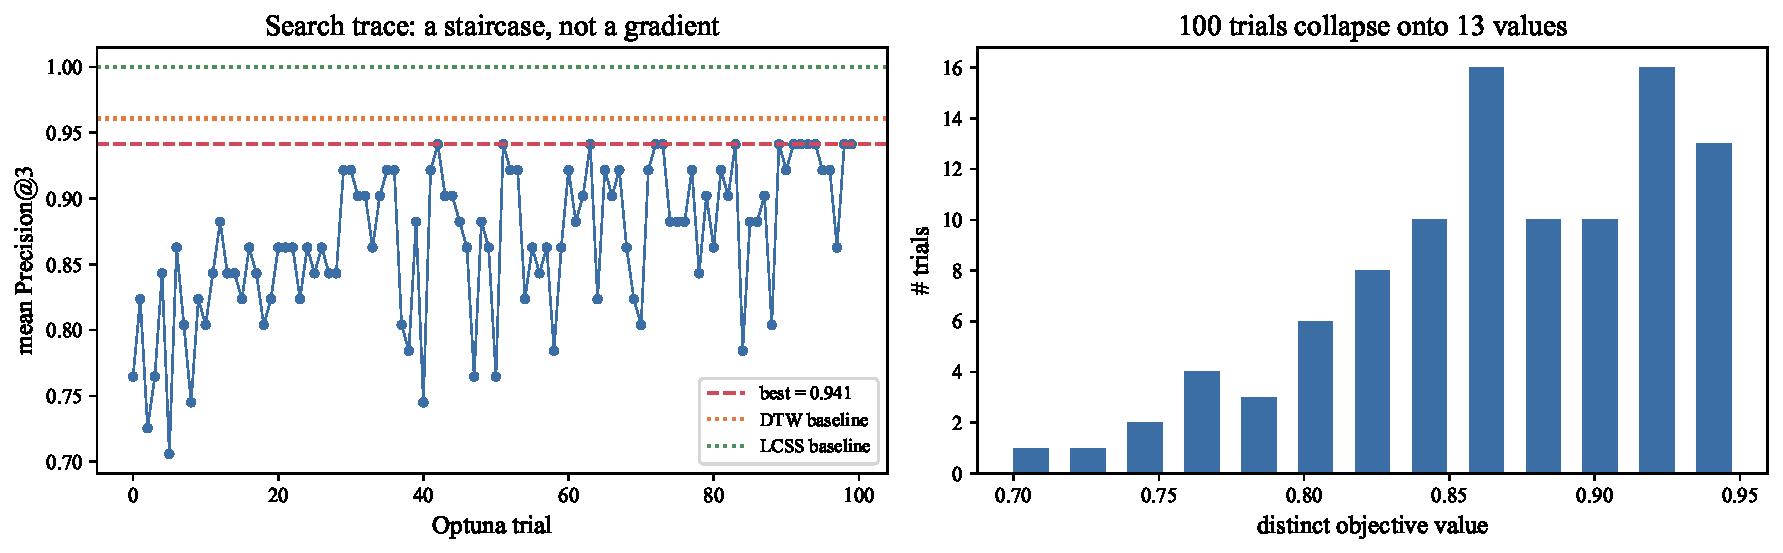
\includegraphics[width=0.92\textwidth]{figs/fig_tuning_plateau.pdf}
\caption{The recorded tuning run. Left: trial trace against the DTW and LCSS baselines.
Right: 100 trials collapse onto 13 objective values.}
\label{fig:plateau}
\end{figure}

\subsection{Remedy: make the metric a model}
\begin{enumerate}[leftmargin=*]
  \item \textbf{Adopt a comparison likelihood.} For anchor $a$ and candidates $b,c$, model
  $\Pr(b\text{ preferred}) = \sigma\big((d_\vartheta(a,c)-d_\vartheta(a,b))/\tau\big)$ ---
  the Bradley--Terry / triplet-logistic form [14] --- and maximise the log-likelihood. It is
  continuous, uses every comparison instead of a top-$k$ count, is calibrated, and makes
  $\tau$ an explicit annotator-noise parameter (per-annotator temperatures or a random effect
  handle disagreement). This alone removes the plateau of (a).
  \item \textbf{Make $d_\vartheta$ differentiable and widen $\vartheta$.} With the soft-min
  DP of \S\ref{sec:merge}, gradients reach $\rho$, $\beta$, the weights, and the segmentation
  $\lambda$: every hand-set constant becomes a fitted parameter. [11] gives the smoothing and
  its gradient; [12] generalises to arbitrary DPs, which the merge-aware recursion needs.
  \item \textbf{Replace diagonal weights with a low-rank metric}
  $d^2 = (x-y)^\top M(x-y)$, $M = A^\top\!A$, $A\in\mathbb{R}^{r\times12}$, $r\approx4$
  [17]. This is the correct response to collinearity: learn the directions that matter rather
  than weighting correlated features independently. Whiten on the segment corpus first and
  regularise $M$ toward the identity for identifiability.
  \item \textbf{Fix the protocol.} Grouped $k$-fold CV by anchor; a held-out test set never
  touched during development; bootstrap CIs over anchors; baselines on the same folds; report
  effective ($w^2$) importances.
\end{enumerate}

\paragraph{On annotation size.} 17 anchors cannot support 12 parameters, let alone a metric
matrix. Either \textbf{collect adaptively} --- the adversarial mining already picks
informative comparisons, so formalise it as active learning, with acquisition criteria from
the crowd-kernel / ordinal-embedding literature [15,16] --- or \textbf{shrink the model}: fit
only $\rho$, $\beta$, $\tau$ by maximum likelihood and derive the rest. Three identifiable
parameters fitted honestly is publishable; twelve unidentifiable ones tuned on the training
set is not.

\paragraph{Establish the ceiling.} Fit a free ordinal embedding (t-STE [15], crowd kernel
[16]) to the same triplets. It has no interpretability but bounds what \emph{any} model can
achieve here and measures annotation consistency. ``The interpretable metric attains $x\%$ of
achievable agreement'' is a far stronger claim than an unbounded accuracy number, and guards
against the case where the annotations are too noisy to separate any two methods.

% ===============================================================
\section{Additional defects found during the audit}
\label{sec:cross}
% ===============================================================

\paragraph{Merging on standardised features is algebraically wrong.}
\code{extract\_segment\_features} returns $z = (\phi-m)/\sigma$;
\code{merge\_segments\_features} then \emph{sums} the $z$-scores of the additive features
(\code{sum\_abs\_diff}, \code{length}, and \code{amplitude} for same-sign segments). But
$z(\phi_1)+z(\phi_2) \neq z(\phi_1+\phi_2)$ --- the gap is a constant $m/\sigma$ per extra
merged segment: \code{length} 1.370 s.d.\ (\finding{4.11} at a 4-way merge),
\code{sum\_abs\_diff} 1.021 (3.06), \code{amplitude} 0.994 (2.98). A merged node is pushed
several standard deviations from every unmerged node purely by bookkeeping, regardless of its
shape. Since merging \emph{is} the contribution, this is the most consequential defect found.
\textbf{Fix:} merge in raw space, standardise after. Note weights are also applied \emph{before}
the merge (\code{seq\_sim\_alg.py:74--75}).

\paragraph{Standardisation constants are unattributed.} The 12 means and s.d.s at
\code{utils.py:332--337} are literals; no script in the repository computes them. Recompute
on the current corpus, check the computation in, and refresh whenever the segmenter changes
--- which it will, under \S\ref{sec:cpd}.

\paragraph{Dead and vestigial code.} Besides \S\ref{sec:cpd}(d): \code{mark\_nodes\_limits}
(\code{utils.py:253}) is never called and contains an \code{if start == 760: pass} stub;
\code{dtw\_merge} has \code{if i == 4 and j == 4 ...: pass} at \code{utils.py:413}.

% ===============================================================
\section{Prioritised roadmap}
\label{sec:roadmap}
% ===============================================================

\begin{table}[H]
\centering\small
\caption{Recommendations by impact per unit of effort.}
\begin{tabularx}{\textwidth}{clXcc}
\toprule
\# & \S & Action & Effort & Impact \\
\midrule
1 & \ref{sec:cross} & Merge in raw space, standardise after (removes a multi-s.d.\ artefact from the core operation) & S & Critical \\
2 & \ref{sec:learning} & Grouped cross-validation + held-out test set; re-report all numbers & S & Critical \\
3 & \ref{sec:cpd} & Delete or wire in the dead extremum branch; re-run all results & S & High \\
4 & \ref{sec:cross} & Recompute standardisation constants from the corpus, in a checked-in script & S & High \\
5 & \ref{sec:scale} & Dimensionless features + explicit aspect ratio $\rho$; verify resampling invariance & M & High \\
6 & \ref{sec:cpd} & Replace the detector with $\ell_1$ trend filtering or PELT; add the stability metric & M & High \\
7 & \ref{sec:merge} & Merge penalty $\beta$ from reconstruction residual; bound \code{max\_merge} to 3--4 & M & High \\
8 & \ref{sec:learning} & Bradley--Terry likelihood over annotator comparisons & M & High \\
9 & \ref{sec:learning} & Soft-min DP; fit $\rho,\beta,\lambda,w$ by gradient descent & L & High \\
10& \ref{sec:scale} & Low-rank Mahalanobis metric in place of diagonal weights & L & Medium \\
11& \ref{sec:learning} & Ordinal-embedding ceiling (t-STE) to bound achievable agreement & M & Medium \\
12& \ref{sec:merge} & Benchmark against shapeDTW / SSDTW & M & Medium \\
\bottomrule
\end{tabularx}
\end{table}

\vspace{-0.5em}
Items 1--4 are corrections, not redesigns; do them first, since every current number depends
on them and item 1 may change the method's standing against the baselines. Items 5--8 are the
redesign and are mutually reinforcing --- dimensionless features make the aspect ratio
meaningful, a principled segmenter makes the merge residual computable, and a differentiable
cost makes all of it learnable from the annotations already being collected. Item 9 unifies
them.

% ===============================================================
\section*{References}
\addcontentsline{toc}{section}{References}
% ===============================================================
{\small
\begin{enumerate}[leftmargin=*,itemsep=0pt,parsep=0pt,label={[\arabic*]}]
\item F.-l. Chung, T.-c. Fu, R. Luk, V. Ng. ``Flexible time series pattern matching based on
perceptually important points,'' \emph{IJCAI Workshop on Learning from Temporal and Spatial
Data}, 2001.
\item E. Keogh, S. Chu, D. Hart, M. Pazzani. ``Segmenting time series: a survey and novel
approach,'' in \emph{Data Mining in Time Series Databases}, World Scientific, 2004.
\item C. Truong, L. Oudre, N. Vayatis. ``Selective review of offline change point detection
methods,'' \emph{Signal Processing}, 167:107299, 2020. (\code{ruptures}.)
\item R. Killick, P. Fearnhead, I. A. Eckley. ``Optimal detection of changepoints with a
linear computational cost,'' \emph{JASA}, 107(500):1590--1598, 2012.
\item P. Fearnhead, G. Rigaill. ``Changepoint detection in the presence of outliers,''
\emph{JASA}, 114(525):169--183, 2019.
\item S.-J. Kim, K. Koh, S. Boyd, D. Gorinevsky. ``$\ell_1$ trend filtering,'' \emph{SIAM
Review}, 51(2):339--360, 2009.
\item D. H. Douglas, T. K. Peucker. ``Algorithms for the reduction of the number of points
required to represent a digitized line or its caricature,'' \emph{Cartographica},
10(2):112--122, 1973.
\item S. Gharghabi, Y. Ding, C.-C. M. Yeh, K. Kamgar, L. Ulanova, E. Keogh. ``Matrix Profile
VIII: Domain agnostic online semantic segmentation at superhuman performance levels,''
\emph{ICDM}, 2017.
\item T. Rakthanmanon, E. Keogh, S. Lonardi, S. Evans. ``MDL-based time series clustering,''
\emph{Knowledge and Information Systems}, 33(2):371--399, 2012.
\item J. Zhao, L. Itti. ``shapeDTW: Shape Dynamic Time Warping,'' \emph{Pattern Recognition},
74:171--184, 2018.
\item M. Cuturi, M. Blondel. ``Soft-DTW: a differentiable loss function for time-series,''
\emph{ICML}, 2017.
\item A. Mensch, M. Blondel. ``Differentiable dynamic programming for structured prediction
and attention,'' \emph{ICML}, 2018.
\item G. E. A. P. A. Batista, E. J. Keogh, O. M. Tataw, V. M. A. de Souza. ``CID: an
efficient complexity-invariant distance for time series,'' \emph{DMKD}, 28(3):634--669, 2014.
\item R. A. Bradley, M. E. Terry. ``Rank analysis of incomplete block designs: I. The method
of paired comparisons,'' \emph{Biometrika}, 39(3/4):324--345, 1952.
\item L. van der Maaten, K. Weinberger. ``Stochastic triplet embedding,'' \emph{MLSP}, 2012.
\item O. Tamuz, C. Liu, S. Belongie, O. Shamir, A. T. Kalai. ``Adaptively learning the crowd
kernel,'' \emph{ICML}, 2011.
\item K. Q. Weinberger, L. K. Saul. ``Distance metric learning for large margin nearest
neighbor classification,'' \emph{JMLR}, 10:207--244, 2009.
\item W. S. Cleveland, M. E. McGill, R. McGill. ``The shape parameter of a two-variable
graph,'' \emph{JASA}, 83(402):289--300, 1988.
\item J. Talbot, J. Gerth, P. Hanrahan. ``An empirical model of slope ratio comparisons,''
\emph{IEEE TVCG}, 18(12):2613--2620, 2012.
\item A. Gogolou, T. Tsandilas, T. Palpanas, A. Bezerianos. ``Comparing similarity perception
in time series visualizations,'' \emph{IEEE TVCG}, 25(1):523--533, 2019.
\item M. Vlachos, G. Kollios, D. Gunopulos. ``Discovering similar multidimensional
trajectories,'' \emph{ICDE}, 2002.
\item H. Sakoe, S. Chiba. ``Dynamic programming algorithm optimization for spoken word
recognition,'' \emph{IEEE TASSP}, 26(1):43--49, 1978.
\end{enumerate}
}

\end{document}
